\documentclass[a4paper, 12pt]{article}
\usepackage{amsmath}
\usepackage{graphicx}
\usepackage{caption}
\usepackage{float}
\usepackage{minted}
\usepackage{xcolor}
\definecolor{LightGray}{gray}{0.9}
\usepackage{ragged2e}

\title{STK1100 - Obligatorisk oppgavesett 2 av 2}
\author{Klaudia M. Pawlak}
\date{07.05.2020}
\begin{document}
\maketitle

\section*{Oppgave 1}
\begin{FlushLeft}
La \( X \) være årsinntekten til en tilfeldig valgt person i en befolkningsgruppe, og \( \kappa \) være minsteinntekten i denne gruppen. La \( \theta > 2 \) være en parameter som avhenger av lønnsforskjellene i gruppen.
\end{FlushLeft}
\subsection*{a)}
Vi har at \( X \) har sannsynlighetstettheten
\[
f_X(x) = 
\begin{cases} 
\theta \kappa^\theta x^{-\theta-1}, & \text{for } x > \kappa \\
0, & \text{ellers}
\end{cases}
\]
Vi vil finne den kumulative sannsynlighetsfordelingen \( F_X(x) \) til \( X \). Denne er definert som
\[
F_X(x) = P(X \leq x) = \int_{-\infty}^{x} f_X(y) \, dy
\]
Vi setter den nedre grensen til \( \kappa \), og vi får
\[
F_X(x) = \int_{\kappa}^{x} f_X(y) \, dy = \int_{\kappa}^{x} \theta \kappa^\theta y^{-\theta-1} \, dy = \theta \kappa^\theta \int_{\kappa}^{x} y^{-\theta-1} \, dy
\]
\[
= \theta \kappa^\theta \left[ \frac{y^{-\theta}}{-\theta} \right]_{\kappa}^{x} = 1 - \kappa^\theta x^{-\theta}
\]
\begin{FlushLeft}
For å finne median årsinntekt setter vi
\end{FlushLeft}
\[
F_X(m) = \frac{1}{2}
\]
og får
\[
\frac{1}{2} = 1 - \kappa^\theta m^{-\theta}
\]
Vi løser denne ligningen for \( m \) og får
\[
m = \kappa \sqrt[\theta]{2}
\]

\subsection*{b)}
Vi skal finne forventet årsinntekt \( E(X) \). Vi har at
\[
E(X) = \int_{\kappa}^{\infty} x f_X(x) \, dx = \int_{\kappa}^{\infty} x \theta \kappa^\theta x^{-\theta-1} \, dx
\]
\[
= \theta \kappa^\theta \int_{\kappa}^{\infty} x^{1-\theta-1} \, dx = \frac{\theta \kappa}{\theta - 1}
\]

\subsection*{c)}
Median årsinntekt blir: 
\[
m = \sqrt[3]{2} \cdot 400000 = 503968.42
\]
Forventet årsinntekt blir 
\[
E(X) = \frac{3 \cdot 400000}{3 - 1} = 600000
\]
I motsetning til gjennomsnittet blir medianen mindre påvirket av svært høye eller lave inntekter, og gir derfor et mer nøyaktig mål på hva som er typisk for gruppen.

\subsection*{d)}
Variansen er definert som
\[
V(X) = E((X - \mu)^2) = E(X^2) - \mu_X^2
\]
Og standardavviket er definert som
\[
\sigma_X = \sqrt{V(X)}
\]
Vi regner ut \( V(X) \)
\[
V(X) = \int_{\kappa}^{\infty} \theta \kappa^{\theta} x^{-\theta+1} \, dx - (\frac{\theta \kappa}{\theta - 1})^{2}
\]
\[
= \int_{\kappa}^{\infty} \theta \kappa^{\theta} x^{-\theta+1} \, dx - \frac{\theta^{2} \kappa^{2}}{(\theta - 1)^{2}}
\]
Integralet blir
\[
\int_{\kappa}^{\infty} \theta \kappa^{\theta} x^{-\theta+1} \, dx = \frac{\kappa^{2}\theta x^{2-\theta}}{2-\theta} + C
\]
Så det bestemte integralet blir
\[
V(X) = \frac{\kappa^{2}\theta}{\theta - 2} - \mu_X^2
\]
Og vi får
\[
V(X) = \frac{\kappa^{2-\theta}}{\theta - 2} - \mu_X^2 = \frac{\kappa^{2}\theta}{(\theta - 2)(\theta - 1)^{2}}
\]
Og
\[
\sigma_X = \sqrt{(\frac{\kappa^{2}\theta}{(\theta - 2)(\theta - 1)^{2}})}
\]

\subsection*{e)}
Vi lar \( Y = \theta \ln\left(\frac{X}{\kappa}\right) \). Deretter uttrykker vi \( X \) ved hjelp av \( Y \):
\[
X = \kappa e^{\frac{Y}{\theta}}
\]
Vi finner sannsynlighetstettheten til \( Y \):
\[
f_Y(y) = f_X\left(\kappa e^{\frac{y}{\theta}}\right) \cdot \left|\frac{d}{dy}\left(\kappa e^{\frac{y}{\theta}}\right)\right|
\]
\[
= \theta \kappa^\theta \left(\kappa e^{\frac{y}{\theta}}\right)^{-\theta-1} \cdot \frac{1}{\theta} e^{\frac{y}{\theta}}
\]
\[
= \frac{1}{\kappa} e^{-y}
\]
Dette viser at \( Y \) følger en eksponentialfordeling.

\section*{Oppgave 2}
\subsection*{a)}
Vi har en simultan sannsynlighetstetthet
\[
f(x, y) = 
\begin{cases} 
k(x + 2y), & \text{for } 0 \leq x \leq 1, 0 \leq y \leq 1, x + y \leq 1 \\
0, & \text{ellers}
\end{cases}
\]
hvor \( k \) er en konstant. Vi skal vise at \( k = 2 \). For å finne \( k \) kan vi bruke at denne fordelingen skal være normalisert, altså
\[
\iint_D k(x + 2y) \, dx \, dy = 1
\]
hvor \( D \) er området definert av \( 0 \leq x \leq 1 \), \( 0 \leq y \leq 1 \), og \( x + y \leq 1 \). Vi regner ut integralet:
\[
\int_0^1 \int_0^{1-x} k(x + 2y) \, dy \, dx = 1
\]
Vi integrerer først med hensyn på \( y \):
\[
\int_0^{1-x} k(x + 2y) \, dy = k \left[xy + y^2\right]_{0}^{1-x} = k\left[x(1-x) + (1-x)^2\right]
\]
Deretter integrerer vi med hensyn på \( x \):
\[
\int_0^1 k\left[x(1-x) + (1-x)^2\right] \, dx = 1
\]
Etter utregning finner vi at \( k = 2 \).

\subsection*{b)}
Vi skal finne \( P(Y \leq X) \). Området hvor \( Y \leq X \) er området der \( y \) varierer fra 0 til \( x \). Dette betyr at
\[
P(Y \leq X) = \iint_{D'} k(x + 2y) \, dy \, dx
\]
hvor \( D' \) er området definert av \( 0 \leq y \leq x \) og \( 0 \leq x \leq 1 \). Vi setter inn verdien for \( k \):
\[
P(Y \leq X) = \int_0^1 \int_0^x 2(x + 2y) \, dy \, dx
\]
Vi integrerer først med hensyn på \( y \):
\[
\int_0^x 2(x + 2y) \, dy = 2\left[xy + y^2\right]_{0}^{x} = 2(x^2 + x^2) = 2x^2
\]
Deretter integrerer vi med hensyn på \( x \):
\[
\int_0^1 2x^2 \, dx = \left[\frac{2x^3}{3}\right]_{0}^{1} = \frac{2}{3}
\]
Derfor er \( P(Y \leq X) = \frac{2}{3} \).

\subsection*{c)}
Vi vil finne den marginale sannsynligheten til \( X \). Vi får
\[
f_X(x) = \int_0^{1-x} k(x + 2y) \, dy
\]
\[
= k\left[x(1-x) + (1-x)^2\right]
\]
Ved forenkling finner vi
\[
f_X(x) = 2(x + 1) \quad \text{for} \quad 0 \leq x \leq 1
\]

\subsection*{d)}
Den marginale sannsynligheten til \( Y \) blir
\[
f_Y(y) = \int_0^{1-y} k(x + 2y) \, dx
\]
\[
= k\left[\frac{(1-y)^2}{2} + 2y(1-y)\right]
\]
For alle andre tilfeller vil \( f_Y(y) = 0 \). Etter forenkling, finner vi:
\[
f_Y(y) = 1 + 4y \quad \text{for} \quad 0 \leq y \leq 1
\]

\subsection*{e)}
Vi ser at \( f_X(x) \cdot f_Y(y) \neq f(x, y) \). Derfor er de ikke uavhengige.

\section*{Oppgave 3}
Vi bruker Python og skriver denne programmet for de neste oppgavene:

\begin{minted}
[
bgcolor=LightGray,
fontsize=\footnotesize,
linenos
]
{python}
import numpy as np
import matplotlib.pyplot as plt

k = 400000
t = 3

def F_invers(x):
    return k/(1 - x)**(1/t)

def f(x):
    return t*k**t*x**(-t - 1)

n = 10000
u = np.random.uniform(0, 1, n)
p = F_invers(u)

print("median = %f" %(np.median(p)))
print("gjennomsnitt = %f" %(np.mean(p)))

x = np.linspace(k, 2000000, n)
tetthet = f(x)

plt.xlim(300000,2000000)
plt.hist(p, density=True, edgecolor="black", bins=300)
plt.plot(x, tetthet)
plt.xlabel("Årsinntekt")
plt.ylabel("Sannsynlighet")
plt.show()
\end{minted}

\subsection*{a)}
Se Python-programmet

\subsection*{b)}
Se Python-programmet

\subsection*{c)}
Kjøreeksempel av Python-programmet gir:
\begin{figure}[h]
    \centering
    
\includegraphics[width=0.5\linewidth]{figure1.jpg}
\end{figure}
\[
\text{Median} = 506625.06 \quad \text{og} \quad E(X) = 602336.49
\]
\begin{FlushLeft}
Det er kun små avvik i resultatene.
\end{FlushLeft}
\subsection*{d)}
Se Python-programmet. Kjøreeksempel gir:
\begin{figure}[h]
    \centering
    
\includegraphics[width=0.5\linewidth]{figure2.jpg}
    \caption{Histogram}
    \label{fig:enter-label}
\end{figure}

\subsection*{e)}
Se Python-programmet. Kjøreeksempel gir:
\begin{figure}[h]
    \centering
    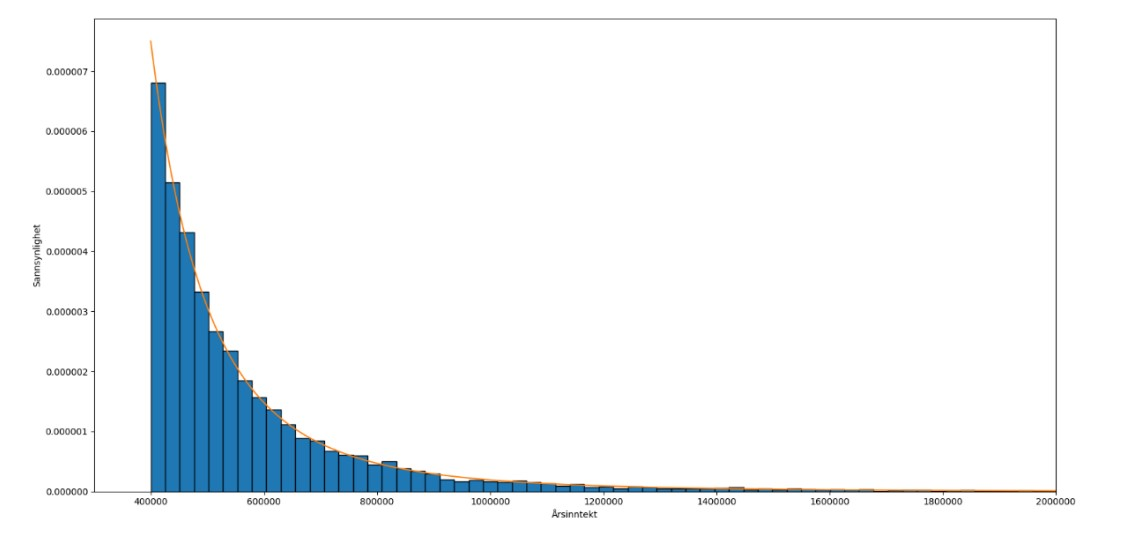
\includegraphics[width=0.5\linewidth]{figure3.jpg}
    \caption{Histogram og tettheten}
    \label{fig:enter-label}
\end{figure}

\end{document}
